\documentclass[11pt]{article}
\usepackage[utf8]{inputenc} % Pour les caractères accentués
\usepackage[french]{babel} % Pour la langue française
\usepackage{hyperref} % Pour les liens cliquables dans le PDF
\usepackage{titlesec} % Pour personnaliser les titres
\usepackage{graphicx}







% Supprime "Chapitre" et garde juste le numéro
\titleformat{\chapter}[hang]
    {\normalfont\huge\bfseries}
    {\thechapter.}
    {0.5em}
    {}

\title{Rapport du projet de Java : Gestion des budgets d'une bville}
\date{}
\author{Feryel BENAMEUR, Lucie BOUCHERON, Clara BAIGNERES}

\begin{document}
\maketitle

\tableofcontents

\section{Introduction}


Dans le cadre de notre cours “Java-Objet”, nous devions réaliser un projet qui avait pour objectif de modéliser et de simuler le fonctionnement d’une équipe municipale. Cette équipe était chargée de proposer, évaluer et sélectionner des projets, puis de résoudre un problème de sac à dos multidimensionnel à l’aide de méthodes gloutonnes. L’ensemble du code Java a été réalisé sous Eclipse. Le travail de groupe a pu être effectué via GitHub et l’utilisation de git grâce à un système de branches.

\subsection{La répartition du travail}

Ce travail qui avait pour vocation de gérer les budgets d’une ville ainsi que les projets d’une équipe municipale à été réalisé en plusieurs étapes. 

Dans un premier temps, BENAMEUR Féryel a construit un schéma sous forme de modèle UML (cf annexe) et a pris en charge le développement du package équipe. Elle a ainsi créé les différentes classes permettant la simulation d’une équipe municipale.

Parallèlement, BAIGNÈRES Clara s’est chargée du package solveurGlouton et ainsi d’implémenter les classes utiles à l’implémentation de méthodes gloutonnes. De son côté, BOUCHERON Lucie a réalisé le package SacADos et donc la construction des classes sac à dos et objets.

Dans un second temps, Féryel s’est occupée de construire la classe Main puis Clara l’a reprise afin de la rendre intéractive.

Enfin, dans un dernier temps, les tests JUnits ont été effectués par Féryel. La rédaction du rapport ainsi que la Javadoc ont été assurés par les trois membres du groupe.

\subsection{Présentation globale de la structure de notre code}
Notre code se découpe en quatre parties qui peuvent être décrites comme suit : 
\begin{enumerate}
	\item Le package équipe : simulation d’une équipe municipale et simulation de projet
	\item Le package sacADos : implémentation d'un sac à dos multidimensionnel et d'objets
	\item Le package solveurGlouton : génère des solutions gloutonnes 
\end{enumerate}

\section{Le package equipe }
Dans la première partie du projet, il nous était demandé de construire un package équipe qui avait pour vocation de construire notre équipe municipale et, par la suite, de créer et proposer des projets, notamment par certains membres municipaux. 

Ce package comprend donc toutes les classes utiles ainsi que leurs constructeurs nécessaires à la création de notre équipe municipale. 

Les getters et setters (utilisés par d’autres classes) nous permettent d’accéder et de modifier les attributs privés de nos classes. 

\subsection{La classe Personne}
Nous avons tout d’abord commencé par réaliser une classe mère nommée "Personne" après avoir constaté que les Élu, Experts et Évaluateurs étaient avant tout des personnes. Nous avons donc utilisé la notion d’héritage pour ces quatre classes afin d’éviter de rappeler le nom, prénom et âge de la personne en question. La classe Personne est donc une classe mère qui a pour but de construire les individus de notre équipe municipale.

\subsection{La classe Expert}
Cette classe fille héritée de la classe Personne a pour objectif de créer nos experts qui, rattachés à un (ou des) secteur(s), ont les compétences pour proposer des projets. 


\subsubsection{La méthode proposerProjets}
Cette méthode crée un projet par secteur rattaché à un élu (avec un titre et une description).

Cette méthode affiche ensuite dans la console le projet proposé. Elle renvoie une liste de tous les projets proposés par l'expert. 

\subsection{La classe Evaluateur}
Cette classe fille héritée de la classe Personne a pour objectif de créer nos évaluateur qui, rattachés à un type d’évaluation du coût, ont les compétences pour déterminer le coût d’un projet.

\subsubsection{La méthode évaluerCoutProjet}
Cette méthode attribue un coût  au projet en fonction du type de l’évaluateur : 
\begin{itemize}
	\item Si l'évaluateur est économique, il fixe un coût économique aléatoire allant de 5000 à 10000.
	\item S’il est social, il fixe un coût social aléatoire allant de 5000 à 10000.
	\item S'il est environnemental, il fixe un coût environnemental aléatoire allant de 5000 à 10000.
\end{itemize}

\subsection{La classe Elu}
Cette classe fille héritée de la classe Personne a pour objectif de créer nos élus municipaux qui estiment le bénéfice d’un projet.

\subsubsection{La méthode estimerBenefice}
Cette méthode calcule le bénéfice d’un projet pour l’élu de manière aléatoire. Elle prend en paramètre un projet et lui assigne une valeur de bénéfice générée automatiquement. 

\subsection{La classe Cout}
Cette classe représente les coûts (économique, social et environnemental) associés à un projet. Ce sont les coûts qui sont évalués par nos évaluateurs. 

\subsubsection{La méthode ToArray}
Cette méthode convertit les différents coûts du projet en un tableau d’entiers. Chaque case du tableau représente respectivement le coût économique, social et environnemental.

\subsubsection{La méthode getCoutTotal}

Parallèlement aux autres coûts nous avons construit cette méthode qui nous permet de renvoyer le coût total du projet comme étant la somme de nos trois coûts. 

Si l’un des coûts n’a pas été évalué et n’est donc pas connu (valeur -1), cette méthode nous affiche une erreur pour empêcher un calcul incorrect.


\subsection{L’énumération Secteur}
Cette énumération regroupe l’ensemble des secteurs auxquels un projet municipal peut être rattaché : sport, santé, éducation, culture, attractivité économique et écologie.

\subsection{L’énumération TypeEvaluationCout}
Cette énumération regroupe l’ensemble des types d’évaluation auxquels peuvent être spécialisés les évaluateurs : économique, social et environnement.

\subsection{La classe Projet}

Cette classe représente les différents projets proposés par les membres de l’équipe municipale.

\subsubsection{La méthode getCoutTotal}
Cette méthode calcule le coût total du projet en additionnant les différents coûts évalués. Seules les valeurs positives ou nulles sont prises en compte afin d’ignorer les coûts non définis ou négatifs.

\subsubsection{La méthode toString}
Méthode qui renvoie une représentation textuelle dans la console du projet. Cette méthode permet ainsi d’afficher facilement toutes les informations essentielles (titre, description, coût et secteur(s)) d’un projet.

\subsection{La classe Équipe Municipale}

\subsubsection{La méthode executerUnCycleDeSimulation}

Cette méthode réalise un cycle de simulation des projets en commençant par examiner les projets proposés par les experts. 

Si aucun projet n’a encore été étudié, chaque expert dans notre liste propose un projet pour chacun de ses secteurs. Les trois évaluateurs attribuent respectivement le coût économique, social et environnemental. L’élu estime enfin le bénéfice du projet, avant que celui-ci ne soit ajouté à la liste des projets étudiés.
\section{Le package solveurGlouton}
\subsection{La classe Utils}
La classe Utils nous permet de définir des méthodes classiques que l’on utilisera au fil de la création de nos autres classes afin de les alléger.

\subsubsection{addCoordinates}
Permet de sommer les éléments de deux tableaux, indice par indice. Elle renvoie une erreur si on essaye de sommer les éléments de deux tableaux de taille différentes. Sinon elle renvoie un nouveau tableau avec le résultat des sommes. 

\subsubsection{substractCoordinates}
À l’inverse de la précédente, cette méthode sert à soustraire les éléments de deux tableaux, indice par indice. Elle renvoie également une erreur si on essaye de soustraire les éléments de deux tableaux de tailles différentes. Sinon elle renvoie un nouveau tableau avec le résultat des différences.

\subsubsection{allSmaller}
Permet de comparer les éléments de deux tableaux et de vérifier que tous les éléments du tableau entré en premier paramètre (dans notre cas le tableau “a”), sont inférieurs aux éléments du deuxième tableau entré en paramètre (le tableau “bounds”), indice par indice. Comme les méthodes précédentes, si on essaye de comparer des tableaux de tailles différentes, la méthode renvoie une erreur. Cette méthode est une méthode booléenne qui va donc retourner “false” si un (ou plusieurs) élément de “a” est supérieur à l’élément de même indice dans “bounds”. 

\subsubsection{maxValue}
Permet de trouver la valeur maximale dans un tableau entré en paramètre. On définit le maximum de départ (“currentMax”) comme étant le premier élément du tableau. On le compare au suivant. Si celui-ci est plus élevé on remplace notre currentMax par cette nouvelle valeur, sinon on conserve la précédente, et ainsi de suite jusqu’à avoir lu tout le tableau. On renvoie ensuite cette valeur maximale. La méthode renvoie une erreur si le tableau de départ est vide.

\subsubsection{indicesOfValue}
Permet de trouver l’indice (ou les indices, s’il y en a plusieurs) où on retrouve la valeur entrée en paramètre dans un certain tableau. On va donc créer une nouvelle liste “indices”,( dans le cas où il existerait plusieurs indices), et on parcourt le tableau indice par indice. Dès que la valeur du tableau correspond à la valeur recherchée, on ajoute l’indice associé à notre liste. Cette méthode n’a pas besoin de renvoyer une erreur car si le tableau est vide ou que la valeur recherchée n’y est pas, la méthode ne renverra rien. 

\subsubsection{indicesOfMaxValue}
Utilise les deux  précédentes (maxValue et indicesOfValue) pour retrouver la valeur maximale d’un tableau entré en paramètre, puis son (ou ses) indice(s) dans le tableau. Cette méthode renvoie une erreur dans le cas où la méthode “maxValue” renverrait une erreur (i.e. si le tableau d’entrée est vide). 

\subsubsection{sommeDesCouts}
Permet de sommer les coûts de plusieurs objets. On crée donc un tableau “somme” de la taille du nombre de coûts qui existent et on l’initialise à 0. Pour chaque objet dans notre liste entrée en paramètre, on utilise la méthode “addCoordinates” définie plus haut afin de sommer les coûts de “somme” et de notre objet. On obtient donc une nouvelle valeur pour “somme”. La méthode renvoie la somme finale. Elle renvoie une erreur dans le cas où la méthode addCoordinates renvoie une erreur (i.e. lorsque nos deux tableaux sont de tailles différentes).

\subsubsection{utilite}
A pour objectif de nous renvoyer la somme des utilités de tous les objets d’une liste. On initialise donc une variable “utilite” à 0 et, pour chaque objet de notre liste entrée en paramètre, on ajoute à cette variable l’utilité de notre objet. Cette méthode n’a pas besoin de renvoyer d’erreur car si notre liste est vide ou que l’objet n’a pas d’utilité, la méthode ne renvoie rien.


\subsection{L’interface ObjetInterface}
Cette interface précise qu’un objet dans un sac à dos doit contenir une méthode renvoyant son utilité (getUtilite()) et ses coûts calculés par l’évaluateur (getCouts()). 

\subsection{l’interface SacADosInterface}
Cette interface précise qu’un sac à dos possède une méthode qui renvoie sa dimension (getDimension()), les budgets  (getBudgets()) et une liste d’objets issus de mon autre interface ObjetDansSacADos (getObjets()). 
\\

SacADosInterface et un ObjetInterface sont implémentées dans le package sacADos.

\subsection{GloutonAjoutSolver}
Cette classe implémente la résolution du problème de sac à dos multidimensionnel grâce à la méthode gloutonne “par  ajout”. 

\subsubsection{resoudre}
Prend en paramètre un SacADos issu de mon interface. Je récupère une liste d’ObjetInterface et les trie selon un comparateur choisi dans le sujet ($f_\Sigma(o_i) = u_i / (\sum_{\ell=1}^{k}c^\ell_i)$ avec un objet $o_i$ plus interessant que $o_j$ si $f_\Sigma(o_i) ≥ f_\Sigma (o_j)$), qu’on définit dans une nouvelle classe (voir la description de la classe suivante). Une fois nos objets triés, on crée un tableau “conso” de la taille du nombre de nos budgets/coûts par objet qui est initialisée à 0.

On crée ensuite une boucle sur nos objets triés et on crée un tableau “newConso” qui va sommer les coûts de notre objet et “conso” (grâce à addCoordinates). Si toute les valeurs de newConso sont inférieures ou égales aux valeurs de “Budgets” (on vérifie ça grâce à allSmaller de notre classe Utils) notre “newConso” devient notre “conso” et on ajoute l’objet en question à notre liste “result”. On répète cette opérations pour tous les objets 

On renvoie “result” qui contient tous les objets que l’on conserve dans notre sac à dos. 

Nous avons donc une méthode qui, comme demandé dans l’énoncé, trie les objets par ordre décroissant selon une formule proposée, puis ajoute les objets de cette liste à notre sac à dos jusqu’à ce qu' un des budgets soit dépassé au prochain objet. 

(Pour plus d’information sur le code ligne par ligne, voir les commentaires du code)


\subsection{TriParUtiliteSurSommeDesCouts}
Cette classe servira de comparateur pour notre classe GloutonAjoutSolver.

\subsubsection{sommeDesCouts}
Prend en argument un objet issus de ObjetInterface et somme ses coûts dans une même variable nommée “somme”.

\subsubsection{interet}
Calcule l’intérêt d’un objet o entré en paramètre selon la formule choisie : son utilité sur la somme des ses coûts. Elle renvoie le résultat.

\subsubsection{compare}
Compare deux objets o1 et o2 entrés en paramètres, selon leur intérêt calculé grâce à la méthode “intérêt”. Si l'intérêt de o1 est inférieur  à l'intérêt de o2, alors le “return -1” permet de classer l’objet o1 après l’objet o2 dans une liste générée. Si les deux sont égaux, le “return 0” met le premier élément comparé en première position, et enfin si l'intérêt de o1 est supérieure à l'intérêt de o2, le “return 1” classe l’objet o1 avant l’objet o2 dans une liste. Nous avons ainsi une liste triée selon l'intérêt de chacun de nos objets, de manières décroissante. 

\subsection{GloutonRetraitSolver}
Cette classe implémente la résolution du problème de sac à dos multidimensionnel grâce à la méthode gloutonne “par  retrait”.

\subsubsection{resoudre}
Prend en paramètre un SacADos issu de mon interface. Je récupère une liste d’ObjetDansSacADos et les trie selon le comparateur donné dans le sujet ($f_{mv}(o_i) = u_i / \max(\{c_i^\ell, \ell \in L\})$ avec $L \in arg\max_{1≤\ell≤k}(\sum_{o_i \in S}c_i^\ell - b^\ell)$ et un objet $o_i$ est plus intéressant qu'un objet $o_j$ si $f_{mv}(o_i) ≥f_{m}(o_j)$), qu’on définit dans une nouvelle classe (voir la description de la classe “TRiParUtiliteSurCout” plus loin). Une fois nos objets triés, on calcule la consommation courante de tous nos objets grâce à la méthode “consoCourante” décrite juste après. On commence ensuite notre méthode gloutonne : tant que tous nos coûts de consoCourante ne sont pas inférieurs à nos budgets (on utilise la méthode allSmaller de la classe Utils), on retire le premier élément de la liste et on recalcule la “consoCourante”. On crée une liste “objetRetire” pour garder ces éléments retirés. 

Une fois tous les coûts de “consoCourante” inférieurs aux budgets associés, on récupère la liste des objets retirés et on effectue un GloutonAjoutSolver, c’est à dire qu’on trie cette liste par ordre décroissante d'intérêt, puis on vérifie un par un si les éléments peuvent être ajoutés à notre sac à dos tout en respectant les contraintes de budgets. Si oui on l’ajoute, sinon on passe à l’objet suivant.


Nous avons donc une méthode qui trie notre liste d’objets par ordre croissant d'intérêt, qui retire les éléments de la liste jusqu’à ce que la contrainte de budget soit respectée, et qui va ensuite essayer d’ajouter à nouveau certains éléments retirés avec la méthode GloutonAjoutSolver. 

(Pour plus d’information sur le code ligne par ligne, voir les commentaires du code)

\subsubsection{consoCourante}
Cette méthode prend en paramètre une liste d’objets et crée une liste “conso” de la taille du nombre de coûts présent dans un objet, et somme type de coût par type de coûts, tous les coûts des objets de notre liste (dans notre cas on a donc un coût économique, un coût social et un coût environnemental, notre liste “conso” sera de taille trois et on sommera à l’indice 0 tous les coûts économiques de nos objets, à l'indice 1 les coûts sociaux et à l'indice 2 les coûts environnementaux). 

\subsection{TriParUtiliteSurCout}
Cette classe servira de comparateur pour notre classe GloutonRetraitSolver.

\subsubsection{TriParUtiliteSurCout}
Cette méthode calcule la somme des coûts indice par indice auxquels on retranche les budgets associés. Elle va ensuite chercher les indices où on retrouve la valeur maximale de ces résultats. Cela nous permet de paramétrer notre variable indcesMaxValue 

\subsubsection{maxDesCouts}
Cherche le maximum courant parmi les coûts d’un objet. Il renvoie le coût maximal. 

\subsubsection{interet}
Permet enfin de calculer l'intérêt d’un objet selon la formule de l’énoncé : AJOUTER FORMULE EN LATEX (grâce aux deux méthodes definies précédemment). Elle renvoie le résultat de l'intérêt de l’objet

\subsubsection{compare}
Permet de comparer les intérêts de deux objets et de les ordonner du moins au plus intéressant.

\subsection{HillClimbingSolver}
Permet d’implémenter la méthode du HillClimbing (une méthode de recherche locale permettant de trouver une bonne solution à un problème d’optimisation, ou à améliorer une solution d’un problème d’optimisation).

\subsubsection{fonctionHillClimbing}
Prend en paramètre un sacADos et une liste d’objets qui forment la solution initiale. On va venir calculer l’utilité de cette solution initiale (qui est la fonction à maximiser) et créer une liste de tous les objets qui ont été proposés mais pas conservés dans la solution initiale. 

On va maintenant regarder tous les voisins de notre solution initiale et calculer un par un leur utilité. Si elle est meilleure, le voisin devient la nouvelle solution et on regarde tous ses voisins à lui, sinon on passe au voisin suivant. On s’arrête lorsqu’aucun voisin de notre solution n’a une meilleure utilité. 

Pour définir un voisin, on a décidé de dire que S et S’ sont voisins, si et seulement si S est égale à S’ à un objet près. C'est-à-dire qu’on va retirer un objet de S est le remplacer tour à tour par un des objets qui n’ont pas été conservés dans notre solution initiale. Chaque remplacement est un nouveau voisin. On renvoie la liste d'objets formant une solution finale (la solution initiale ou une meilleure solution à un objet près si elle existe). 

\subsubsection{resoudre}
Permet de résoudre la méthode du Hill Climbing classique ainsi que sa variante. Elle prend en paramètre un sacADos et une liste de liste d’objets qui forme l’ensemble des solutions initiales qu’on transmet à notre méthode (chaque solution est une liste, et on crée une liste de ces listes). 

Dans cette méthode, on applique donc à chaque liste de solutions initiales fonctionHillClimbing et on renvoie la meilleure solution trouvée.  


\section{Le package sacADos}
Il nous était demandé de construire un package sacADos qui avait pour but de construire un sac à dos. 
Ce package comprend donc toutes les classes utiles, avec leurs constructeurs, nécessaires à la création  de notre sac à dos. 
Les getters et setters (utilisés par d’autres classes) nous permettent d’accéder et de modifier les attributs de nos classes qui sont privées.

\subsection{La classe Objet}
La classe Objet représente les éléments qui peuvent être mis dans un sac à dos (dans un problème d’optimisation à plusieurs contraintes). Chaque objet possède une utilité et un ensemble de coûts associés aux différents types de coûts représentés dans la classe Cout (dans le package equipe). 

Dans cette classe, on implémente l'interface ObjetInterface pour pouvoir utiliser différents solveurs (définis dans le package solveurGlouton).

\subsubsection{La méthode toString}

Elle renvoie une représentation textuelle dans la console du projet en affichant toutes les informations caractéristiques (utilité et coût(s)) d’un objet.

\subsection{La classe SacADos}
Cette classe représente une implémentation concrète d’un sac à dos. Elle stocke les objets sélectionnés (liste) et les budgets disponibles (tableau) pour la résolution du problème selon les différentes méthodes définies dans l’énumération MethodeDeResolution (ci-dessous).

Elle implémente l’interface SacADosInterface pour garantir la compatibilité avec les différents solveurs.

\subsubsection{La méthode getUtiliteTotale}
Cette méthode calcule la somme des utilités de tous les objets qui sont dans le sac en parcourant simplement la liste des objets et en additionnant leurs utilités.Cela permet d'évaluer la “qualité” d’une solution faite par un des algorithmes de résolution.


\subsubsection{La méthode resoudre}
La méthode resoudre permet de choisir et d’exécuter une des stratégies de résolution parmi celles définies dans l’énumération  (ci-dessous). Elle utilise un switch pour différencier les “comportements” des méthodes. On a donc soit: un appel au solveur glouton par ajout qui va construire une solution, affichée dans la console avec son utilité totale; soit un appel au solveur glouton par retrait; soit aux solveurs Hill Climbing (soit simple, soit multiple).

Cependant, si aucune de ces méthodes de résolution n’est fournie, une exception est levée.

\subsection{L’énumération MethodeDeResolution}
Cette énumération regroupe l’ensemble des méthodes qui peuvent être utilisées pour résoudre un problème de sac à dos, avec une méthode gloutonne basée sur l’ajout successifs d’objets (selon un critère), une cette fois basée sur le retrait et enfin une méthode locale qui explore les solutions voisines pour améliorer sa solution (Hill Climbing simple et multiple).


\section{le package main}

\subsection{La classe VersSacADos}
Cette classe permet de transformer des données issues de projets municipaux ou d’un fichier (MKP) en une structure utilisable dans un problème de sac à dos. Elle permet de construire les tableaux de coûts (sous forme de matrice dans laquelle chaque ligne correspond aux trois coûts d’un objet), de budgets et de bénéfices nécessaires à la création d’un objet dans SacADos.

La classe prend aussi en compte un scénario de conversion grâce à un switch sur l’énumération Scenario : selon le scénario choisi, les coûts des projets sont soit répartis par types de coût (eco, socio, env) soit par secteur (en affectant le coût du projet uniquement à la dimension de son secteur et en mettant les autres dimensions à zéro).

\subsubsection{Le constructeur VersSacADos}
Le constructeur VersSacADos(Path mkpFilePath) lit un fichier MKP et initialise les tableaux de bénéfices, de coûts et de budgets. Il lance une exception si le fichier n’est pas conforme (ex : mauvais nombre de budgets, format incorrect …).

\subsubsection{La méthode genererSacAdos}
Elle permet de créer un objet dans SacADos à partir des données stockées dans la classe. Elle construit une liste d’objets en instanciant un Objet par bénéfice/coûts, puis crée et retourne un sac à dos dans lequel se trouve ces objets et les budgets correspondants.


\subsection{La classe Main}
La classe Main permet de coordonner la simulation des projets municipaux et la résolution du problème par le sac à dos.

\subsubsection{La méthode Main}

Elle commence par demander une graine d’aléa (pour initialiser les tirages aléatoires), puis un scénario qui permet de déterminer et créer la composition des différents acteurs de l'équipe municipale et le type de budget à générer (le scénario par types de coût crée un expert et trois évaluateurs (un par type de coût) et des budgets aléatoires par type alors que le scénario par coûts par secteurs créé quatre experts pour les cinq secteurs et un évaluateur économique, avec des budgets par secteur).

Ensuite, elle lance une simulation complète des projets (via l’objet EquipeMunicipale), qui sont ensuite affichés dans la console. 

Ces projets sont enfin transformés en objets exploitables par un sac à dos à l’aide de la classe ci-dessus et une méthode de résolution est alors choisie via l'énumération MethodeDeResolution.

La solution obtenue est affichée ainsi que son utilité totale.

\subsection{L'énumération Scenario}

Cette énumération définit les deux scénarios possibles pour la simulation des projets municipaux et la création des listes d’évaluateurs, d’experts et des budgets : un basé sur les coûts par types de coûts (eco, socio et env) et l’autre basé sur les coûts par secteur.


\section{Les tests JUnits}

\subsection{EluTest}
Le test unitaire a pour objectif de vérifier que l’élu estime correctement un bénéfice. Pour cela, on a utilisé la méthode AAA (Arrange, Act, Assert) donné en cours. Ainsi, dans ce test on commence par créer un projet et un élu. 

On demande ensuite à l’élu d’estimer le bénéfice du projet à l’aide de la méthode estimerbenefice que l’on souhaite tester dans notre test unitaire. 

Enfin, on s’assure que la valeur estimée est bien comprise entre 0 et 999 conformément au comportement attendu. 

\subsection{EvaluateurTest}
Ce test unitaire a pour objectif de vérifier que l’évaluateur évalue correctement le coût d’un projet en fonction de sa spécialisation. Dans ce test on commence par créer un projet et un évaluateur.

On demande ensuite à l’évaluateur de type économique d’évaluer le coût économique du projet à l’aide de la méthode evaluerCoutProjet que l’on souhaite tester dans notre test unitaire. 

Enfin, on s’assure que la valeur estimée est bien comprise entre 5000 et 15000 conformément au comportement attendu. 

\subsection{Vers SacADosTest}

Ce test unitaire vise à tester deux méthodes tirées de deux cas différents en fonction de si l’on veut transformer un projet en objet de sac à dos dans le cas où les objets sont définis par type de coût ou dans le cas où ils sont définis par le type de secteur. Dans un premier temps, un projet est créé. Ses différents coûts et son bénéfice sont initialisés. 

On applique ensuite la méthode de transformation (transformer les projets en objets de sac à dos) en fonction du scénario sélectionné. 

Enfin, le test s’assure que les coûts du projet sont correctement placés dans le tableau de coûts, soit par type de coûts (économique, social et environnemental), soit par secteurs, conformément au comportement attendu.

\subsection{GloutonRetraitSolveurTest}
Ce test unitaire a pour objectif de vérifier que l’algorithme GloutonRetraitSolver sélectionne correctement les objets les plus utiles tout en respectant la contrainte de capacité du sac à dos. Dans ce test, un sac à dos et plusieurs objets sont créés à l’aide de classes internes. Nous avions construit des classes internes afin de pouvoir instancier des objets et des sac à dos puisque nous avions des interfaces et que l’instanciation d’objet depuis une interface n’est pas faisable sous java. 

Ensuite, l’algorithme est appliqué afin de résoudre le problème. 

Enfin, le test s’assure que le coût total des objets sélectionnés ne dépasse pas le budget disponible et que la solution conserve au moins les objets détenant la plus grande utilité (ceux dont l’utilité est supérieure ou égale à 8 dans notre test), conformément au comportement attendu.

\subsection{HillClimbingSolveurTest}
Ce test unitaire a pour objectif de vérifier que l’algorithme HillClimbingSolver améliore ou conserve la qualité d’une solution initiale valide. Dans ce test, un sac à dos et plusieurs objets sont créés toujours à l’aide de classes internes. De plus, une solution initiale respectant la contrainte de budget est définie. L’algorithme est ensuite exécuté à partir de cette solution. 

Enfin, le test s’assure que la solution finale déterminée par l’utilité finale est au moins aussi bonne que la solution initiale, conformément au comportement attendu.

Un deuxième comportement attendu a été construit. En effet, nous avons considéré que même si une erreur était levée (exception) dans notre algorithme Hill Climbing, notre test ne devait, quant à lui, pas échouer.

\section{Utilisation de l'IA}

Il est important de noter que chaque réponse donnée par l’IA a été résumée ici. Nous avons résumé les points donnés par l’IA qui nous semblait important de mentionner et qui nous ont été utiles dans la procédure de notre projet. Une version non résumé à l’essentiel nous aurait amené à faire des screens très importants pour des affirmations portés par l’IA qui nous étaient d’aucunes utilités.
\\


\textbf{Prompt 1} :  Comment faire pour que mes évaluateurs soient spécialisés sur un type de cout de manière stochastique?

\textbf{Réponse} : Tu créés une seule classe Evaluateur avec un enum TypeEvaluation et tu assignes aléatoirement un type à chaque évaluateur.

Ensuite, quand tu appelles evaluer(projet), l’évaluateur met à jour uniquement son type de coût.   

 =$>$ PS : j’avais déjà créer l’enumeratio grace a une video youtube !
\\

\textbf{Prompt 2} : explique-moi simplement comment savoir quel type d’assert doit- on utiliser dans notre JUnit ?

\textbf{Réponse} : 

\begin{figure}[h]
    \centering
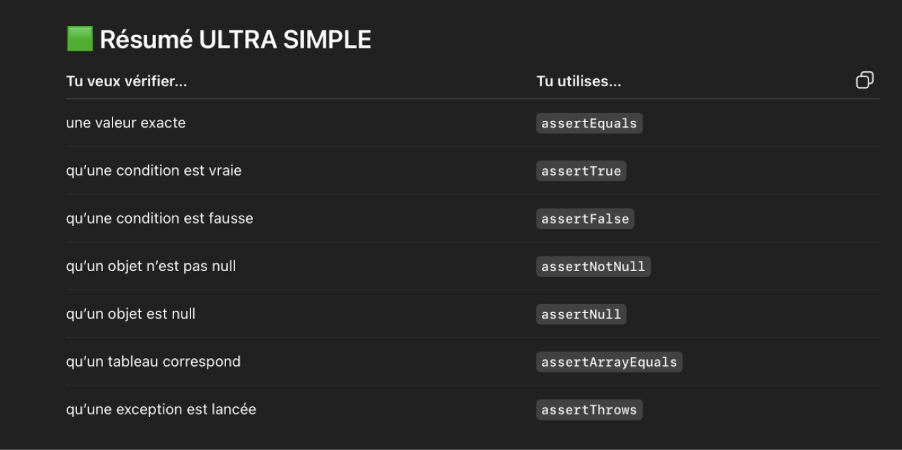
\includegraphics[width=0.6\textwidth]{reponsePrompt2}
\end{figure}


\textbf{Prompt 3} : Voici le code pour GloutonRetraitSolveur. J’ai créé mes objets ainsi que mon sac à dos mais je ne comprends pas comment je peux appliquer le solveur sur ce que j’ai.
\textbf{Réponse} : 
\begin{figure}[h]
    \centering
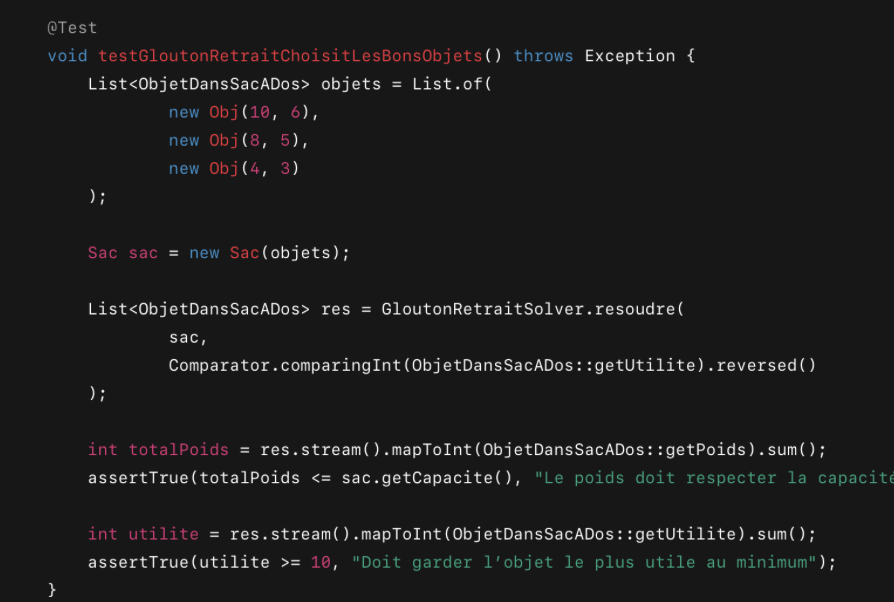
\includegraphics[width=0.6\textwidth]{reponsePrompt3}
\end{figure}


\textbf{Critique} : J’avais déjà instancier les objets et mon sac à dos avec mes objets. j’ai cependant gardé la suite de ce qu’il me donnait dans ce code et l'ai reformulé pour qu’il soit approprié avec ce que j’avais. De plus, il écrivait total Poids au lieu de coutTotal etc.. Donc de nombreuses modifications au niveau syntaxique ont dû être appliquées afin de concorder avec ce qu’on avait. 
\\

\textbf{Prompt 4} : Voici le code pour HillClimbingSolveur. J’ai créé mes objets ainsi que mon sac à dos mais je ne comprends pas comment je peux appliquer le solveur sur ce que j’ai. 

\textbf{Réponse} : 
\begin{figure}[h]
    \centering
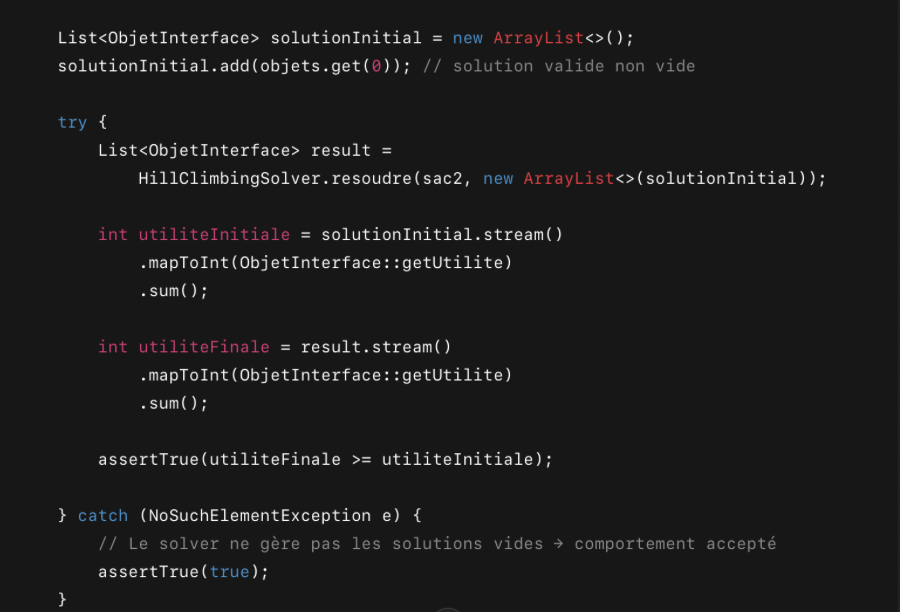
\includegraphics[width=0.6\textwidth]{reponsePrompt4}
\end{figure}

\textbf{Critique} : Tout comme le test pour GloutonRetraitSolveur, j’ai gardé ce qu’il m’avais donné et l’ai un peu adapté en fonction de ce qu’on avait déjà.
\\

\textbf{Prompt 5} : Je ne comprends pas comment faire mon JUnit pour qu’il verifie qu’on a bien changé le coût économique du secteur à son index déterminé. Par exemple, si santé est à l’index 1, comment faire pour qu’il change la valeur de cet index avec le cout économique de ce secteur (pour le JUnit de VersSAcADos).


\textbf{Réponse} : Il me dit qu’il faut utiliser la méthode “.ordinal” pour vérifier le comportement attendus.

\textbf{Critique} : J’ai réutilisé ce qu’il m'a donné en le modifiant avec ce que j’avais. Par exemple, j’ai créé mon projet en fonction du constructeur de la classe projet. Ce code m’a été pratique car j’ai pu l’utiliser pour tester les deux scénarios  en ne changeant presque rien si ce n’est
“Scenario.COUTS\_PAR\_SECTEUR”.

\textbf{Prompt 6 :} How to read of file of "Benchmark instances for the Multidimensional Knapsack Problem" in JAva

textbf{Réponse} : voici un lien vers \href{https://chat.mistral.ai/chat/92226b30-88fe-4807-8545-dee874162ad7}{la réponse}.

\textbf{Critique} : Mistral s’est trompé dans la lecture du fichier. Il me dit que la seconde ligne correspond aux capacités (donc les coûts) de mon premier objets et que les deux dernières lignes sont l’utilité et les budgets. Or le document se découpe comme tel : 
\begin{itemize}
	\item  $n$ le nombre d’objets, $k$ le nombre de budgets, valeur optimale de la solution, $0$ si inconnue.
	\item  Utilité $u_i$ pour chacun des n objets.
	\item  Matrice de contraintes de taille ($k \times n$), i.e., on trouve $c^\ell_i$ à l’indice $[\ell,i]$.
	\item Budget $B^\ell$ pour $\ell \in \{1,...,k\}$.
\end{itemize}
L’utilité est donc en deuxième ligne (et non pas en avant dernière). 

Je me suis donc inspirée de sa réponse pour implémenter un code qui lit le fichier en respectant son architecture.

\section{Ce qui a été dur à implémenter}

\subsection{Pour Feryel}

J’ai eu des difficultés à implémenter les JUnits pour les deux solveurs gloutonnes (GloutonRetraitSolveur et HillClimbingSolveur) car je souhaitais faire un test paramétrés en fonction du fichier téléchargé dans l’énoncé. Cependant, le fichier avait des dimensions trop importantes ou était trop lourd et les solveurs n'arrivaient pas à exécuter les différentes procédures que je souhaitais tester.

Nous avions donc choisi de faire des tests unitaires simples en se basant sur la méthode AAA donnée en cours en construisant des objets et des sac à dos à l’aide de classes internes dans notre JUnit. 

\subsection{Pour Clara}

Ce qui m'a semblé le plus dur dans cet exercice était de respecter et comprendre parfaitement l'architecture du projet. On accumule rapidement plusieurs méthodes dans différentes classes de différents packages, et on s'y perd parfois. 

De plus, l'objectif était de faire dépendre le moins possible un package d'un autre. J'ai donc décidé d'utiliser des interfaces pour mes objets et sac à dos mais il a fallut que Lucie implémente les éléments de mes interfaces pour qu'ils fonctionnent comme je les utilisais dans mon code (ou que je m'adapte moi aussi). 

C'était beaucoup d'allers-retours entre chacun de nos packages et de nos travaux, il a vraiment fallu qu'on soit coordonnées et organisées pour mener à bien ce projet. 


\subsection{Pour Lucie}



\section{Sources}

\begin{itemize}
	\item Toutes la playlist de vidéo Youtube qui suit celle ci (celle ci comprise) : \href{https://youtu.be/VqKZ0tRwUIc?si=KeZxsjvqFKFwB6U-}{liste de vidéos}
	\item \href{https://www.jmdoudoux.fr/java/dej/chap-collections.htm}{https:/www.jmdoudoux.fr/java/dej/chap-collections.htm}
	\item \href{https://openclassrooms.com/forum/sujet/import-classe-java-98358}{https://openclassrooms.com/forum/sujet/import-classe-java-98358}
	\item TP3, TP4 et TP6 du cours de Java Objet de cette année
	\item \href{https://perso.telecom-paristech.fr/hudry/coursJava/tableaux/tableauD.html}{https://perso.telecom-paristech.fr/hudry/coursJava/tableaux/tableauD.html}
	\item \href{https://www.data-transitionnumerique.com/scanner-java/}{https://www.data-transitionnumerique.com/scanner-java/}
	\item \href{https://perso.telecom-paristech.fr/hudry/coursJava/avance/dupliquer.html}{https://perso.telecom-paristech.fr/hudry/coursJava/avance/dupliquer.html}
	\item \href{https://talks.freelancerepublik.com/regles-ecrire-readme-md-github/}{https://talks.freelancerepublik.com/regles-ecrire-readme-md-github/}
	\end{itemize} 
	
	
De plus, le père de Clara nous a aidé à mettre en place une bonne architecture pour le projet et à comprendre certains problèmes de code : indentation, modificateurs d'accès, modificateurs de classe et utilisation d'interfaces, notamment sur glouton pour pouvoir coder parallèlement notre package gloutonSolveur et sacADos.

\section{Annexe (modèle UML)}

\begin{figure}[h]
    \centering
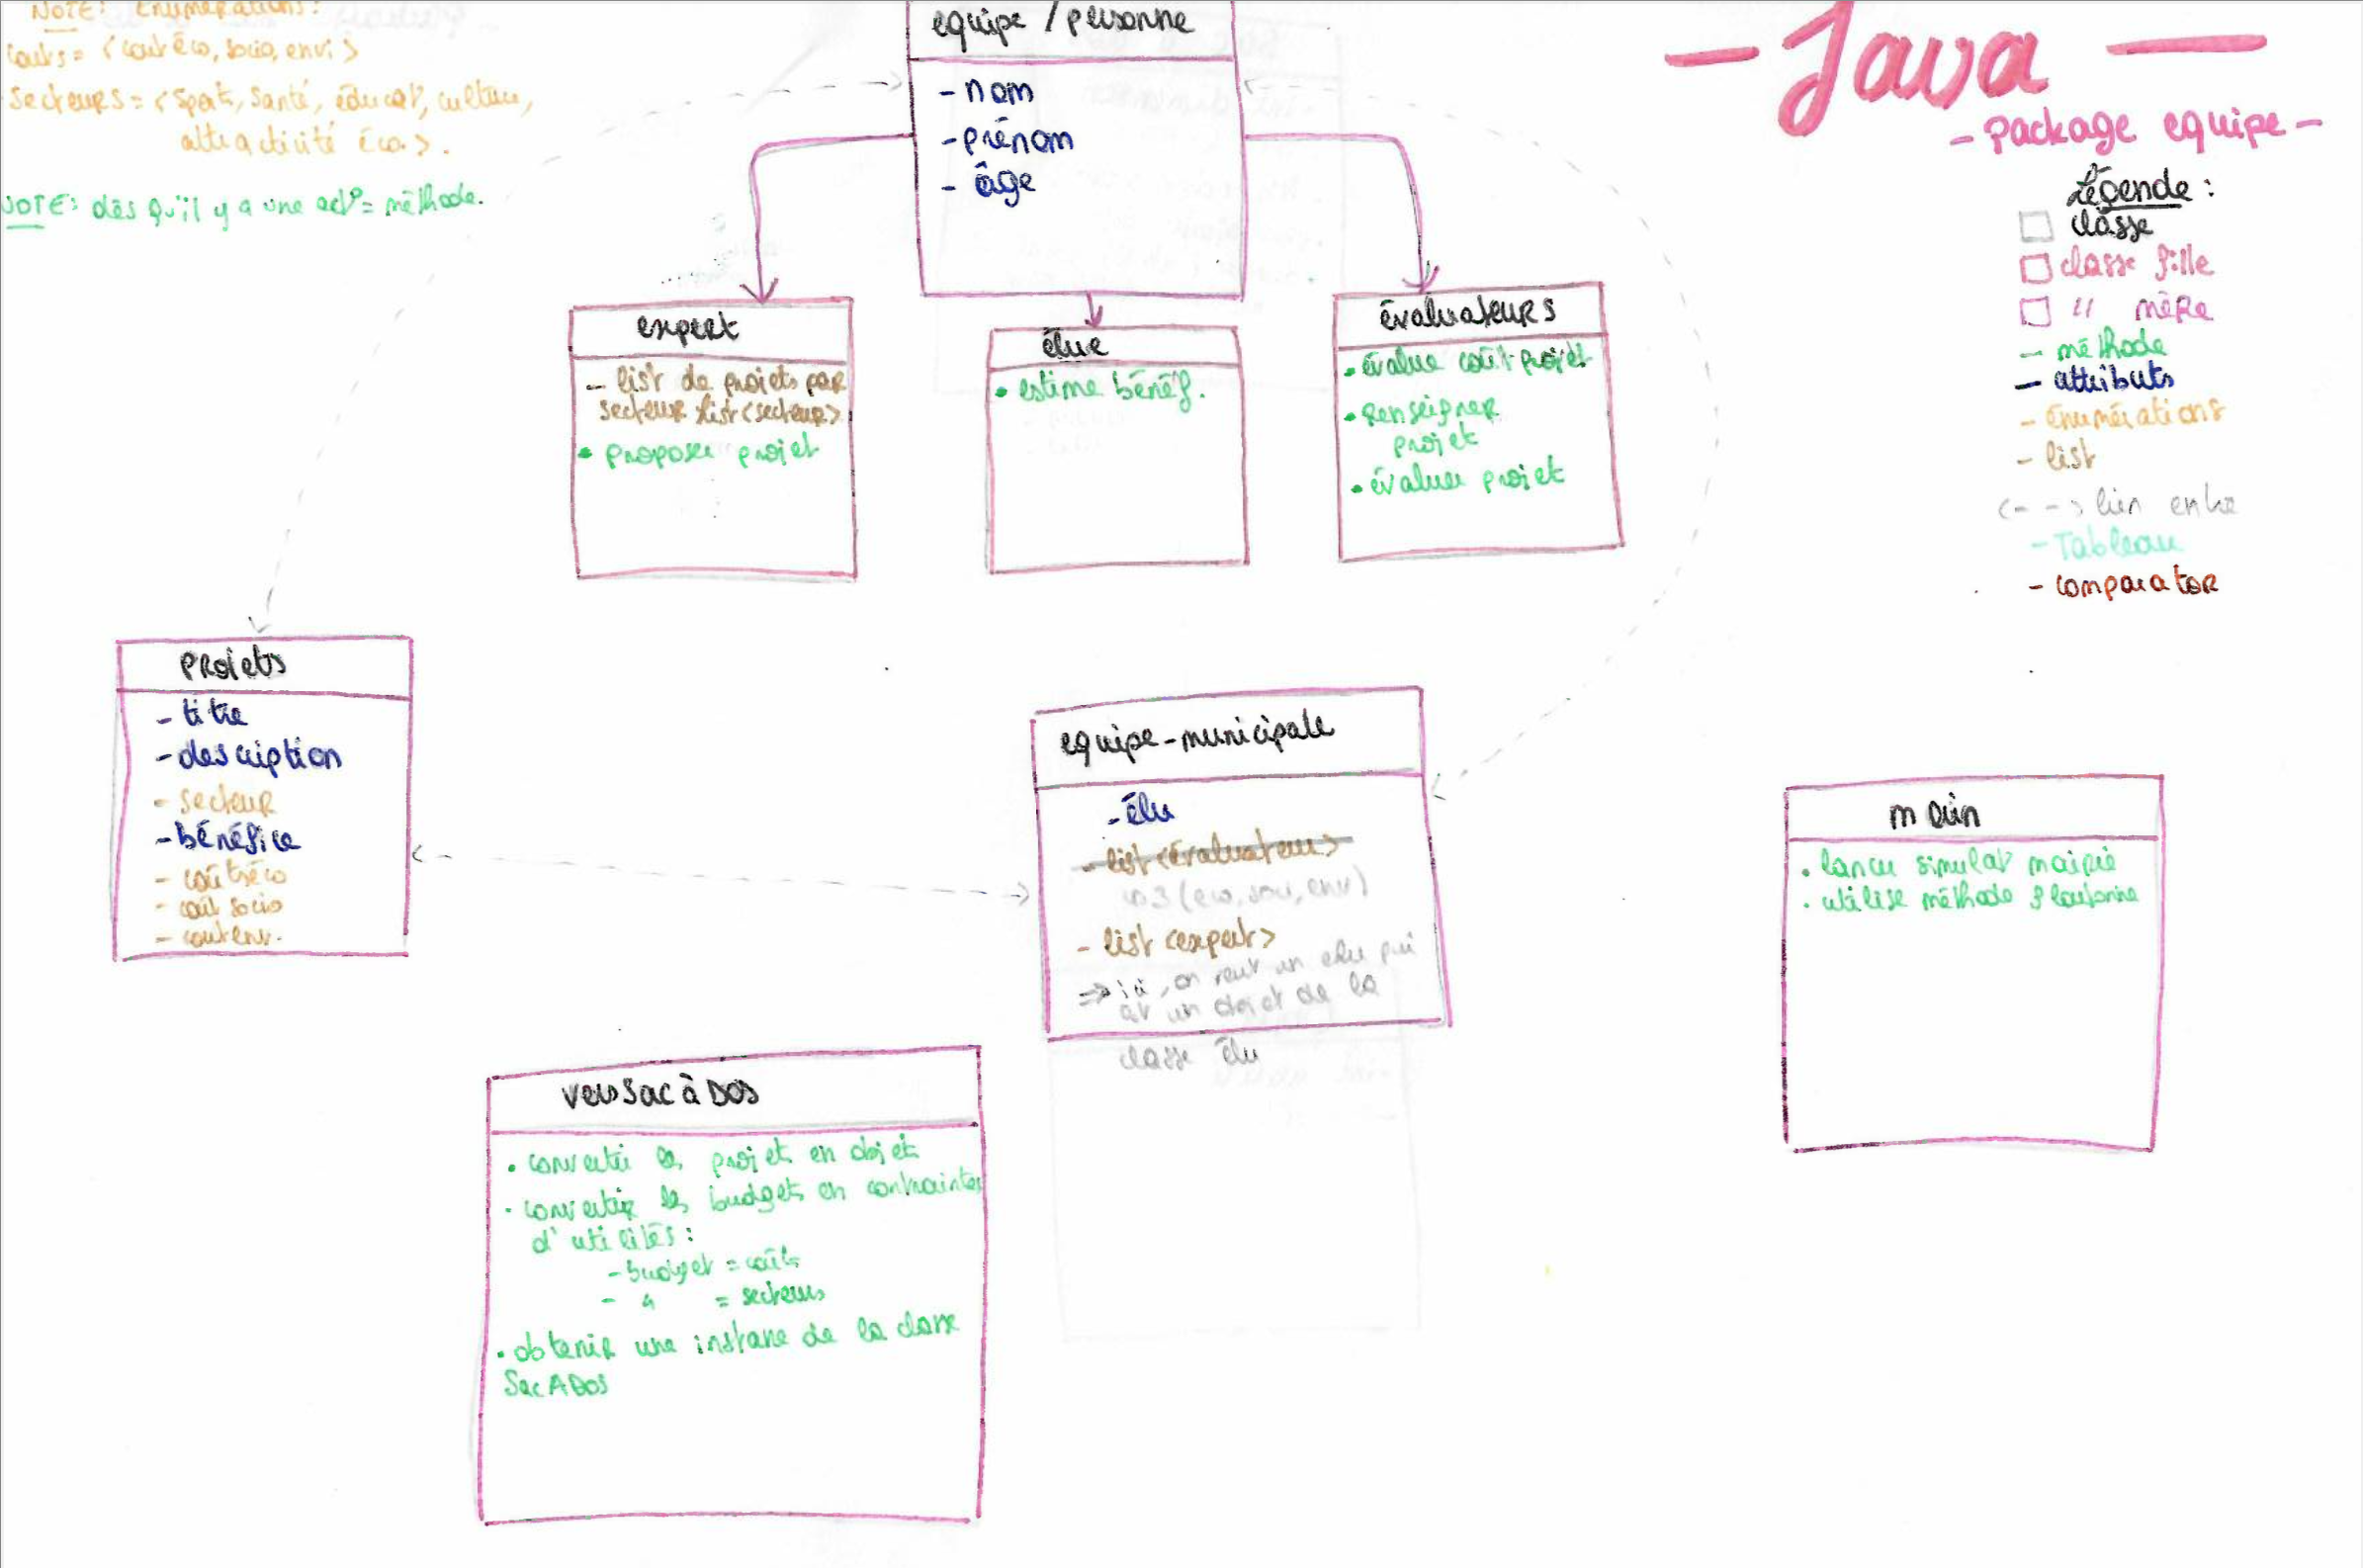
\includegraphics[width=0.7\textwidth]{modeleULM1}
\end{figure}

\begin{figure}[h]
    \centering
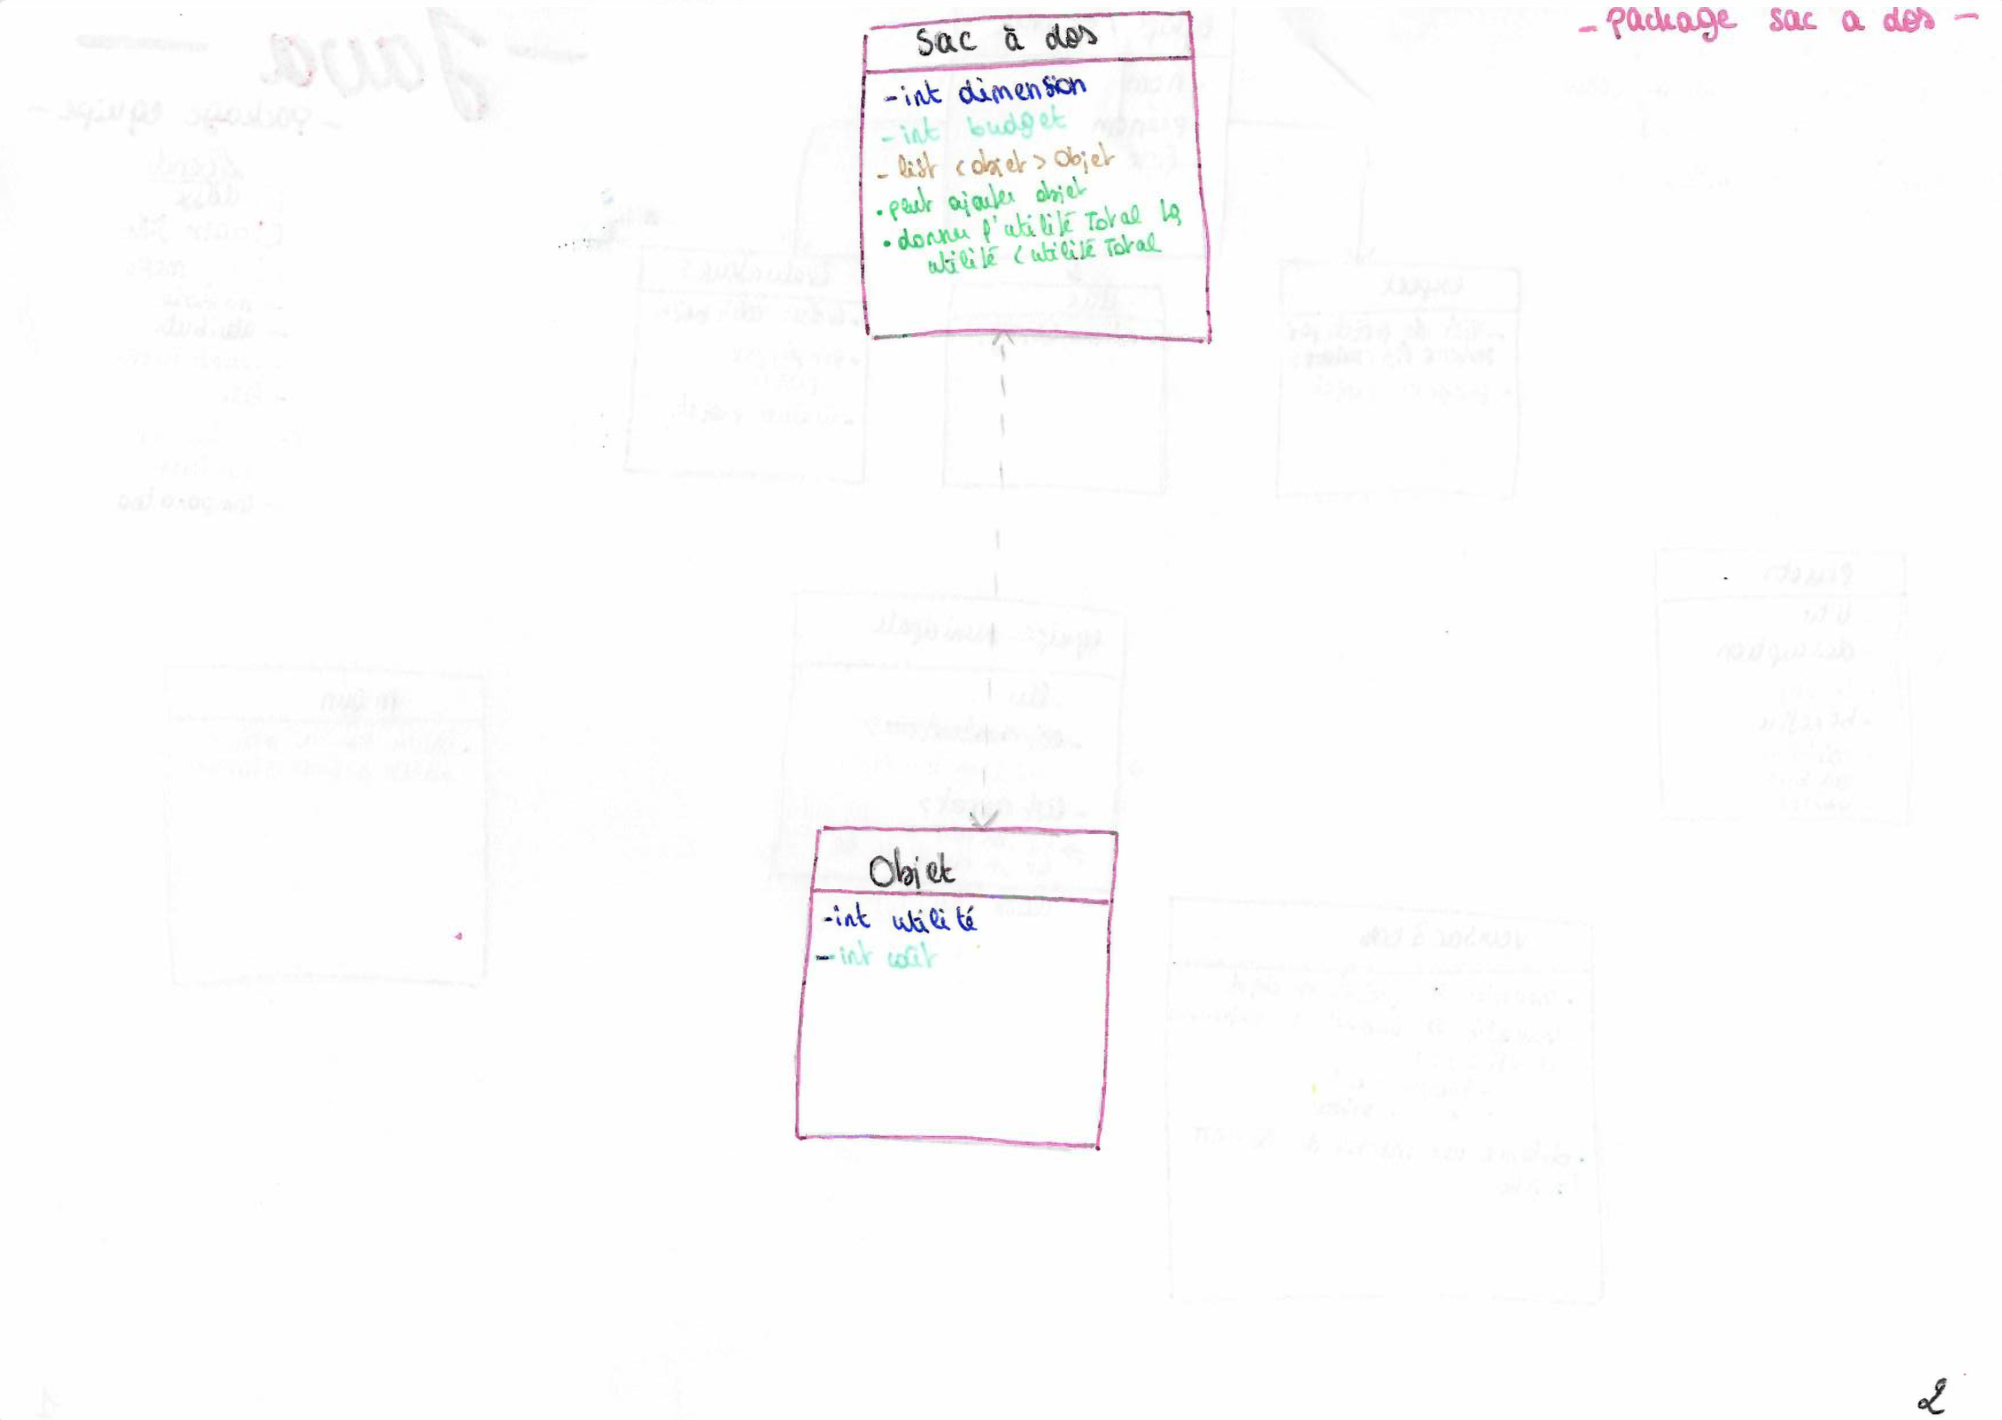
\includegraphics[width=0.7\textwidth]{modeleULM2}
\end{figure}

\begin{figure}[h]
    \centering
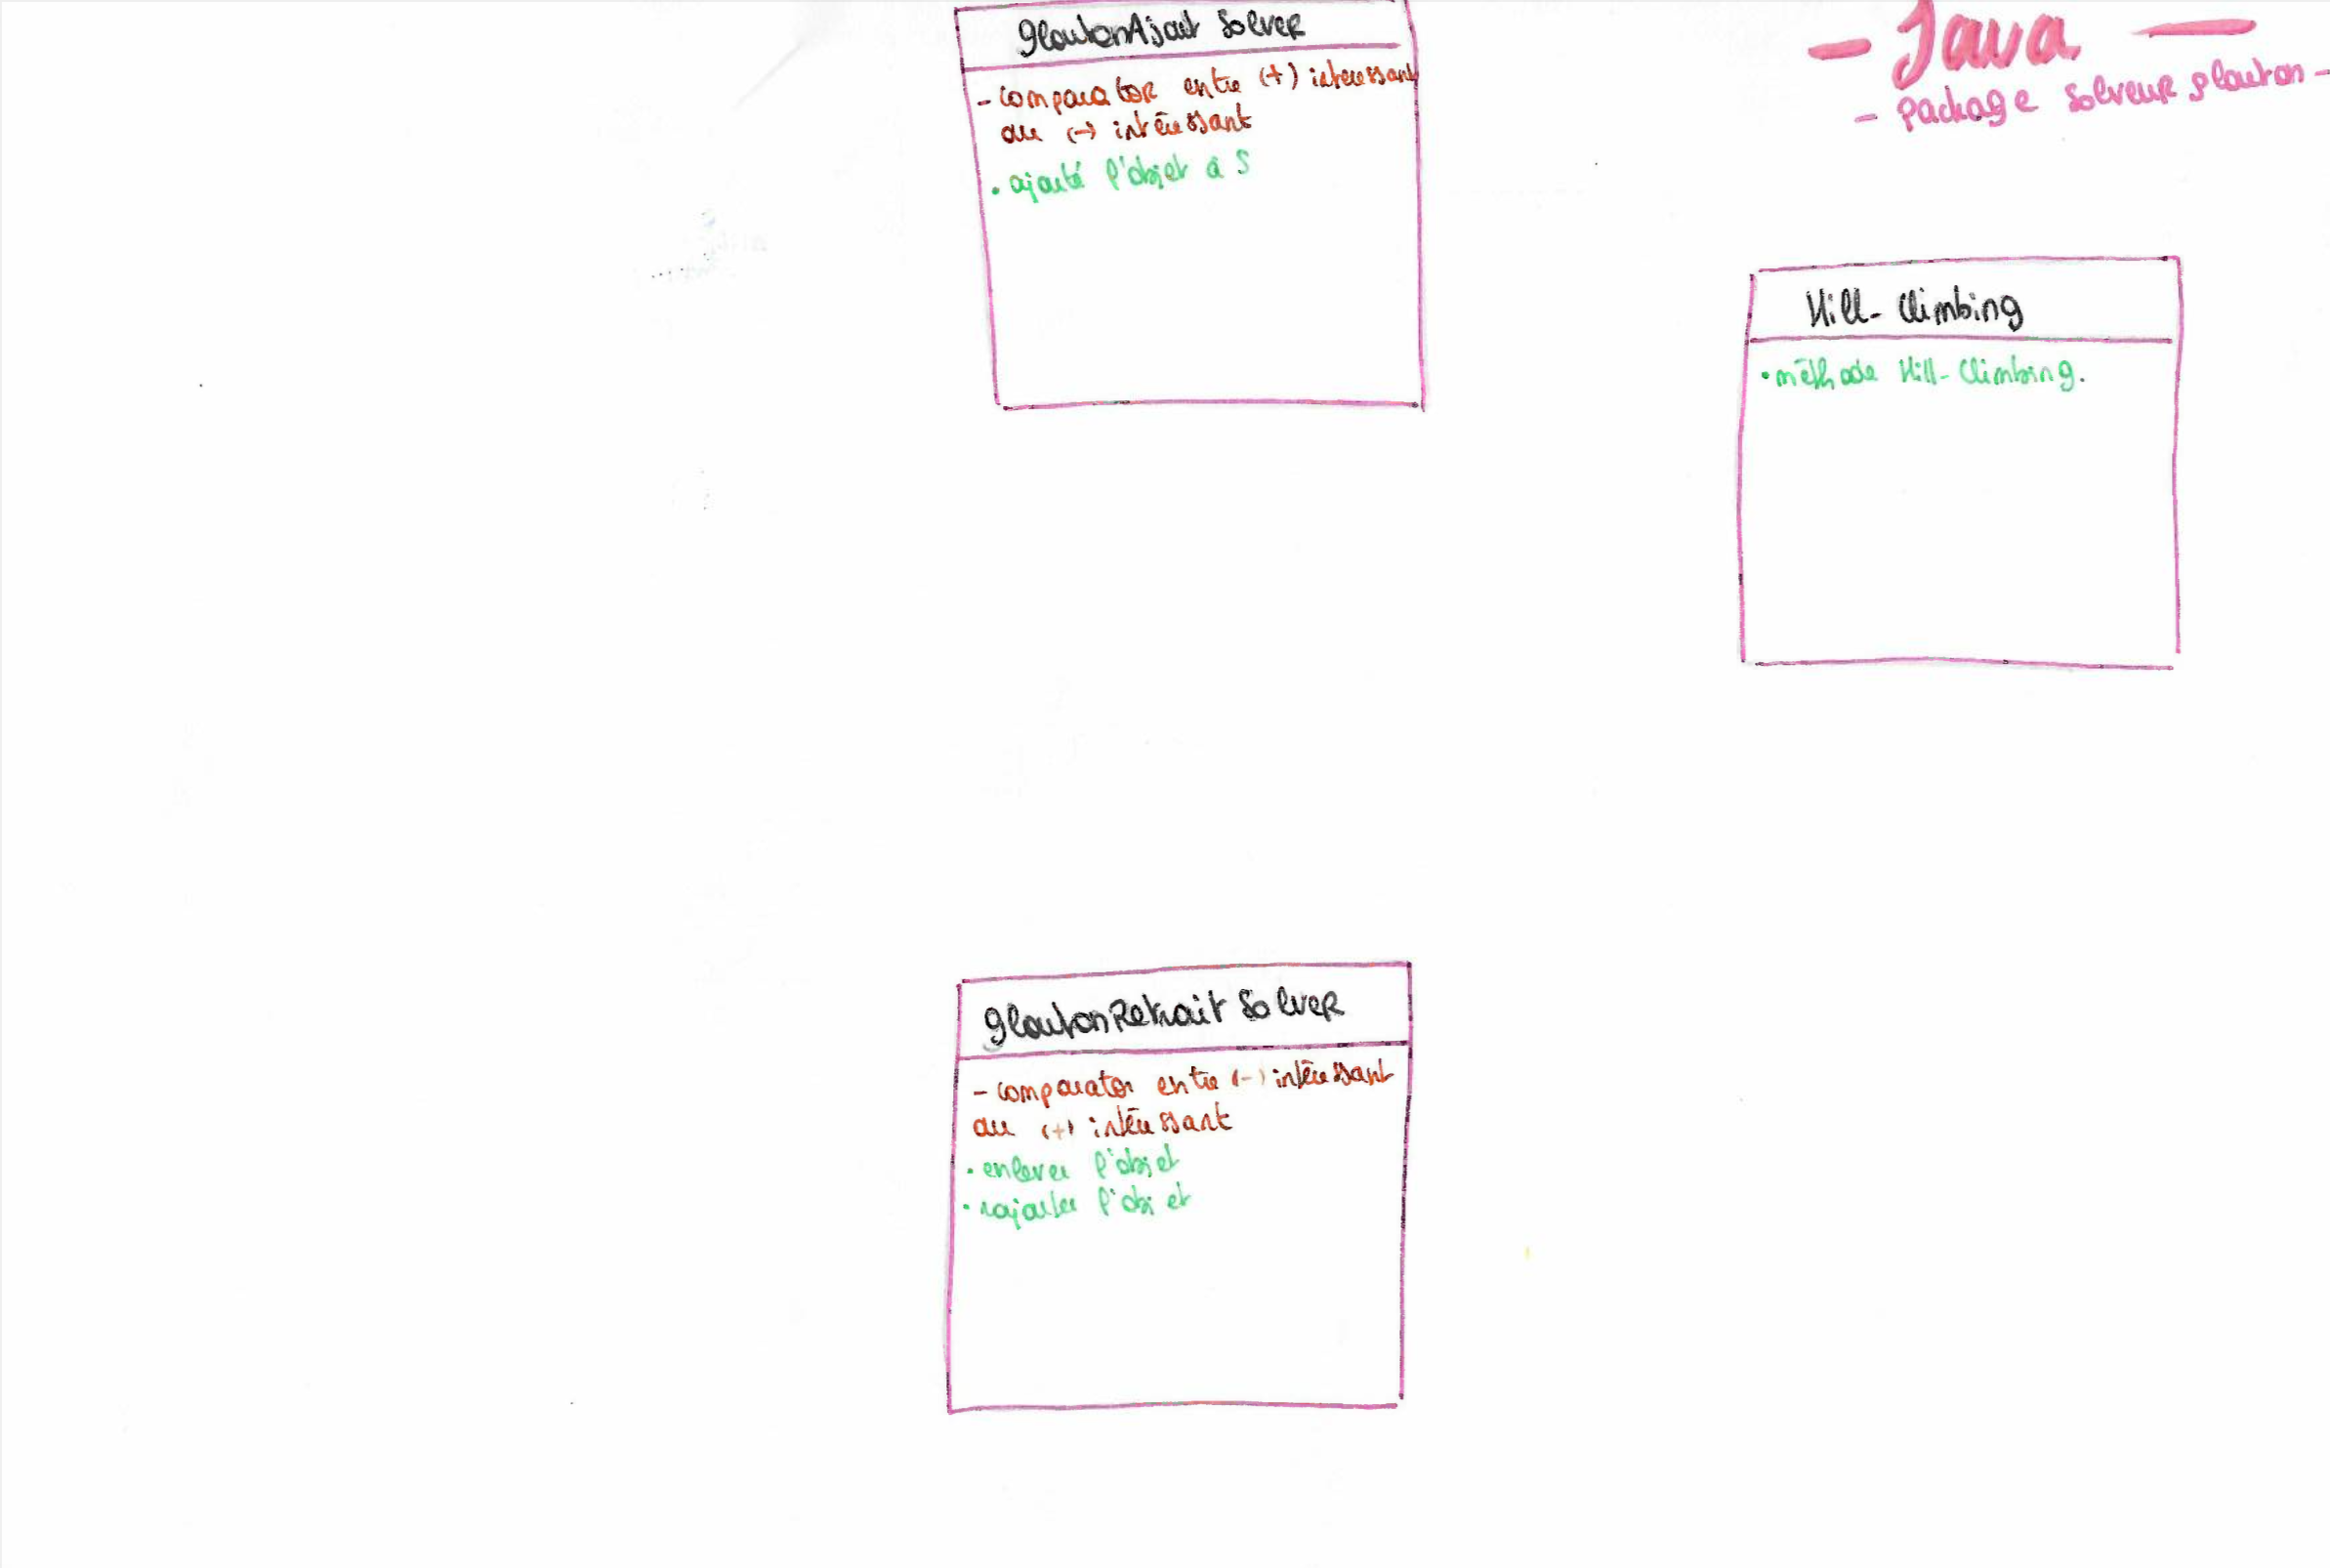
\includegraphics[width=0.7\textwidth]{modeleULM3}
\end{figure}



 





\end{document}
